\documentclass{article}
\usepackage[utf8]{inputenc}
\usepackage{graphicx}
\usepackage[greek,english]{babel}
\usepackage{tikz}
\usepackage{float}
\usepackage{listings}

\title{Εφαρμογή Εξόρυξης και Ανάλυσης Δεδομένων}
\author{}
\date{}

\begin{document}

\maketitle

\section{Σχεδιασμός της εφαρμογής}

\subsection{Επισκόπηση της αρχιτεκτονικής}
Η εφαρμογή έχει σχεδιαστεί ως διαδικτυακή πλατφόρμα με χρήση του Streamlit, το οποίο επιτρέπει την ταχεία ανάπτυξη διαδραστικών εφαρμογών δεδομένων. Η αρχιτεκτονική μπορεί να αναλυθεί σε διάφορα βασικά στοιχεία:

\begin{itemize}
    \item \textbf{Frontend:} Η διεπαφή χρήστη έχει κατασκευαστεί με τη χρήση του Streamlit, παρέχοντας μια διαισθητική και διαδραστική εμπειρία για τους χρήστες για τη μεταφόρτωση δεδομένων, την οπτικοποίηση των αποτελεσμάτων και την εκτέλεση αναλύσεων.
    \item \textbf{Backend:} Το backend αποτελείται από την Python που χειρίζεται τις εργασίες επεξεργασίας δεδομένων, ανάλυσης και μηχανικής μάθησης.
    \item \textbf{Αποθήκευση δεδομένων:} Η εφαρμογή υποστηρίζει τη φόρτωση δεδομένων από διάφορες μορφές, όπως CSV, Excel και TSV.
\end{itemize}

\subsection{Βασικά χαρακτηριστικά}
\begin{itemize}
    \item Φόρτωση δεδομένων
    \item Οπτικοποίηση δεδομένων
    \item Διερευνητική ανάλυση δεδομένων (EDA)
    \item Επιλογή χαρακτηριστικών
    \item Ταξινόμηση μηχανικής μάθησης
    \item Σύγκριση επιδόσεων
\end{itemize}

\subsection{Σχεδιασμός διεπαφής χρήστη}
Η διεπαφή χρήστη περιλαμβάνει:
\begin{itemize}
    \item Widget φόρτωσης αρχείων
    \item Πλοήγηση στην πλαϊνή γραμμή
    \item Διαδραστικά διαγράμματα
\end{itemize}

\section{Εφαρμογή της εφαρμογής}

\subsection{Δομή αποθετηρίου}
\begin{itemize}
    \item \texttt{src/}: Περιέχει τον κύριο κώδικα της εφαρμογής.
    \item \texttt{lib/}: Περιλαμβάνει βιβλιοθήκες και βοηθητικές λειτουργίες.
    \item \texttt{functions/}: Περιέχει ειδικές συναρτήσεις για την επεξεργασία και την ανάλυση δεδομένων.
    \item \texttt{pages/}: Περιέχει διάφορες σελίδες της εφαρμογής Streamlit.
    \item \texttt{Dockerfile}: Χρησιμοποιείται για τη δημιουργία εμπορευματοκιβωτίων της εφαρμογής για εύκολη ανάπτυξη.
\end{itemize}

\subsection{Εγκατάσταση και ρύθμιση}
\begin{lstlisting}[language=bash]
git clone https://github.com/sudo455/texnologia_logismikoy_sptember_2024.git
cd texnologia_logismikoy_sptember_2024/src
python -m venv venv
source venv/bin/activate # Στα Windows, χρησιμοποιήστε venv\Scripts\activate
pip install -r requirements.txt
streamlit run main.py
\end{lstlisting}

\subsection{Βασικές λεπτομέρειες εφαρμογής}
\begin{itemize}
    \item \textbf{Φόρτωση δεδομένων:} Χρήση Pandas για την ανάγνωση αρχείων δεδομένων.
    \item \textbf{Οπτικοποίηση:} Χρήση Matplotlib και Plotly.
    \item \textbf{Μηχανική μάθηση:} Χρήση Scikit-learn.
    \item \textbf{Επιλογή χαρακτηριστικών:} Εφαρμογή τεχνικών όπως η Recursive Feature Elimination (RFE).
\end{itemize}

\subsection{Ανάπτυξη}
\begin{lstlisting}[language=bash]
sudo docker build -t texnologia_logismikoy:latest .
sudo docker run -d -p 8501:80 --name texnologia_logismikoy ghcr.io/sudo455/texnologia_logismikoy:latest
\end{lstlisting}

\section{Συνεισφορές των μελών της ομάδας}

\subsection{Άγγελος Μωραΐτης (inf2021163)}
\begin{itemize}
    \item Φόρτωση δεδομένων
    \item Προεπεξεργασία
    \item Επιλογή χαρακτηριστικών
    \item Αλγόριθμοι ταξινόμησης
\end{itemize}

\subsection{Θεοχάρης Παρίσης (Π2017162)}
\begin{itemize}
    \item Οπτικοποίηση
    \item Μείωση διαστάσεων
    \item Σχεδιασμός UI
    \item Ενσωμάτωση
\end{itemize}

\section{Κύκλος ζωής έκδοσης λογισμικού}

\begin{enumerate}
    \item Σχεδιασμός
    \item Ανάπτυξη
    \item Συνεχής ολοκλήρωση (CI)
    \item Συνεχής παράδοση (CD)
    \item Ανάπτυξη
    \item Ανατροφοδότηση και επανάληψη
    \item Συντήρηση
    \item Τεκμηρίωση
\end{enumerate}

\section{Class Diagram}

\begin{figure}[H]
    \centering
    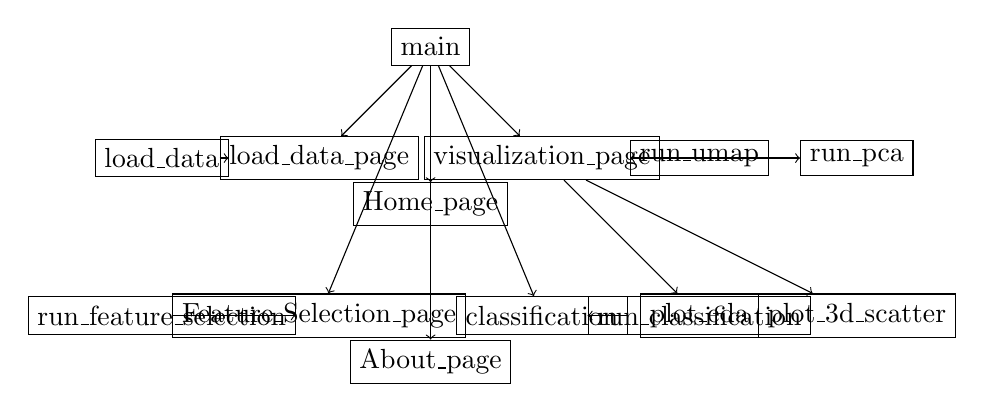
\begin{tikzpicture}[node distance=2cm]
        \node (main) [rectangle, draw] {main};
        \node (home) [rectangle, draw, below of=main] {Home\_page};
        \node (load) [rectangle, draw, below left of=main] {load\_data\_page};
        \node (vis) [rectangle, draw, below right of=main] {visualization\_page};
        \node (feature) [rectangle, draw, below of=load] {Feature\_Selection\_page};
        \node (class) [rectangle, draw, below of=vis] {classification};
        \node (about) [rectangle, draw, below of=home] {About\_page};
        
        \draw[->] (main) -- (home);
        \draw[->] (main) -- (load);
        \draw[->] (main) -- (vis);
        \draw[->] (main) -- (feature);
        \draw[->] (main) -- (class);
        \draw[->] (main) -- (about);
        
        \node (umap) [rectangle, draw, right of=vis] {run\_umap};
        \node (pca) [rectangle, draw, right of=umap] {run\_pca};
        \node (eda) [rectangle, draw, below of=umap] {plot\_eda};
        \node (scatter) [rectangle, draw, below of=pca] {plot\_3d\_scatter};
        
        \draw[->] (vis) -- (umap);
        \draw[->] (vis) -- (pca);
        \draw[->] (vis) -- (eda);
        \draw[->] (vis) -- (scatter);
        
        \node (feature_sel) [rectangle, draw, left of=feature] {run\_feature\_selection};
        \draw[->] (feature) -- (feature_sel);
        
        \node (run_class) [rectangle, draw, right of=class] {run\_classification};
        \draw[->] (class) -- (run_class);
        
        \node (load_data) [rectangle, draw, left of=load] {load\_data};
        \draw[->] (load) -- (load_data);
    \end{tikzpicture}
    \caption{Class Diagram of the Data Mining and Analysis Application}
\end{figure}

\end{document}